\documentclass[../paper.tex]{subfiles}

% Document
\begin{document}
    Last but not least, we will look at machine learning models.
    These are models that are already trained on a lot of data, and can then be used to predict the weather.
    So the hassle of training is already done for us (also in the case of APIs).

    \subsubsection{How does it work?}

    \subsubsection{ClimaX}
        \hfill\\
        ClimaX is the first foundation model designed to perform a wide variety of weather and climate modeling tasks.
        For weather, these tasks include standard forecasting tasks of relevant weather variables like temperature,
        humidity, etc.
        with various lead-times at various resolutions, both globally and regionally.
        For climate, ClimaX can help to make better long-term projections,
        or to downscale lower resolution model outputs to higher resolutions.
        At its core, ClimaX is a multidimensional image-to-image translation architecture based on Vision Transformers
        (ViT).\\
        ViT-based architectures are especially well suited for modeling weather and climate phenomena
        since they naturally tokenize the spatial nature of multiscale data akin to different spatial-temporal inputs.
        Additionally,
        they offer the opportunity to extend tokenization towards a wide range of multichannel features\cite{d1}.
        \\
        \textbf{Results highlights}:\\
            Forecasting the future values of key weather variables at different temporal horizons is critical
            to ensuring the safety of communities and infrastructure around the world.\\
            ERA5 is the latest climate reanalysis produced by ECMWF,
            providing hourly data on many atmospheric,
            land-surface and sea-state parameters together with estimates of uncertainty\cite{d2}. \\
            ERA5 reanalysis data from the ECMWF underlies as the key source of data for training
            and evaluating machine learning models on this task with performance of Operation
            IFS being the current state-of-the art numerical weather prediction baseline.\\
            ClimaX when fine-tuned on the same ERA5 data,
            even at medium resolutions 1.40625\textdegree already performs comparably,
            if not better than IFS on short and medium-range predictions,
            while being substantially better at longer horizon predictions\cite{d1}.
            \begin{figure}[htbp]
            \centerline{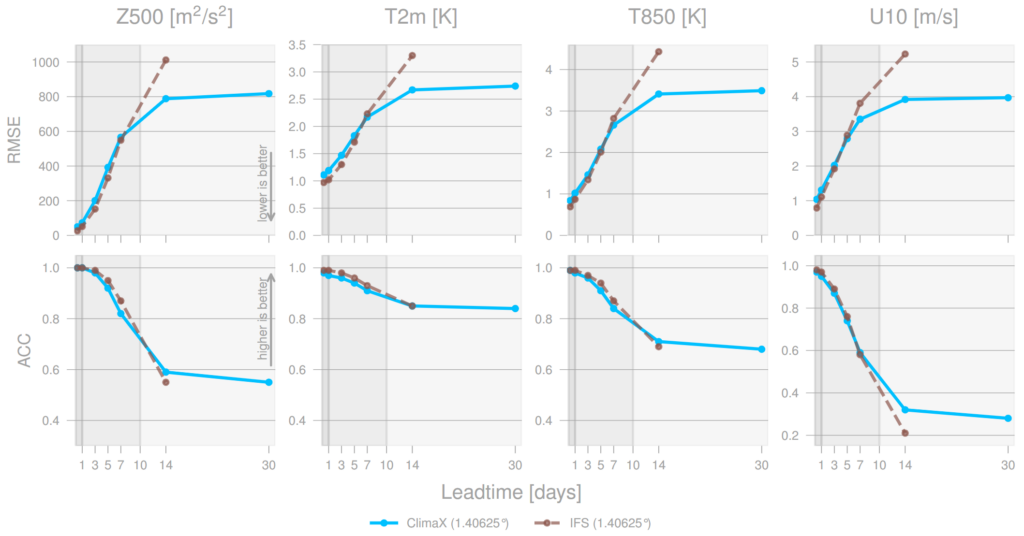
\includegraphics[width=0.5\textwidth]{../photos/climax_ifs}}
            \caption{ClimaX vs IFS on global forecasting of key weather variables at different lead time horizons}
            \label{fig:climax-vs-ifs}
            \end{figure}

            In the graphs above,
            we compare the performance of ClimaX vs IFS on global forecasting of key weather variables at different lead time horizons:
            \begin{itemize}
                \item Temperature T2M (2m above ground)
                \item Temperature T850 (850hPa)
                \item Wind speed U10M (10m above ground)
                \item Geo-potential height Z500 (500hPa)
            \end{itemize}
            The graphs on the first row show the RMSE (root mean squared error) of the predictions,
            while the graphs on the second row show the ACC (accuracy) of the predictions.
            The x-axis shows the lead time in days.
            As we can see, for example, on the Z500 graph, both models start at 100\% accuracy and 0 RMSE.\\
            As the lead time increases, the accuracy of both models decreases, and the error increases.\\
            What a decrease in accuracy means is that the model is less confident in its predictions.\\
            What an increase error means that the model is less accurate and less trustworthy.\\
            For example, on the Z500 graphs, we can see that the accuracy of both models starts at 1.0 (100\%),
            and decreases to around 0.6 (60\%) at 14-days lead time.\\
            At the same time,
            the RMSE of both models starts at 0
            and increases to around 800 for ClimaX and 1000 for IFS at 14 days lead time.
            \\
            But as we can see, ClimaX performs somewhat comparably to IFS on short and medium-range predictions,
            while being substantially better at longer horizon predictions (in most of these graphs, 14 days and above).\\
    \subsubsection{GraphCast}
        GraphCast is a machine learning-based method developed by Google DeepMind for medium-range global weather forecasting.
        It is an autoregressive model based on graph neural networks and a novel high-resolution multiscale mesh representation.
        It is a mesh representation used to represent the Earth's surface and atmosphere.
        The mesh is a grid of points that are connected by lines to form triangles.
        The mesh is multiscale, meaning that it has different resolutions at different levels.
        The mesh is high-resolution, meaning that it has a high density of points, which allows for more accurate predictions.
        GraphCast is trained on historical weather data from the European Centre for Medium-Range Weather Forecasts (ECMWF)'s ERA5 reanalysis archive\cite{e1}.
        \\\\
        It starts with the current state of Earth's weather and data about the weather six hours ago.
        Then, it makes a prediction about what the weather will look like six hours from now.\\
        GraphCast then feeds those predictions back into the model, performs the same calculation, and spits out longer-term forecasts\cite{e1}.\\
        \begin{figure}[htbp]
            \centerline{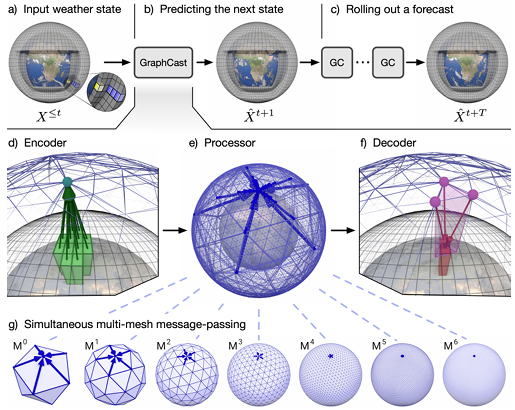
\includegraphics[width=0.4\textwidth]{../photos/multimesh_graphcast}}
            \caption{Steps of GraphCast}
            \label{fig:multimesh-graphcast}
        \end{figure}\\
        GraphCast's multiscale mesh representation. \\
        A) First, we insert the data into the model.
        B) Then we perform GraphCast to predict data, we feed this data back into the model.
        C) We perform GraphCast again to predict data, we feed this data back into the model and do this repeatedly.
        D) The encoder component maps local regions of the input (the green boxes) into nodes of the multi-mesh graph representation.
        E) The processor component performs a series of graph neural network (GNN) message passing steps to update the node features.
        F) The decoder component maps the updated node features back to the output (the purple boxes).
        G) The multi-mesh is a set of icosahedral meshes of increasing resolution, from the base mesh ($M^0$, 12 nodes) to the finest resolution ($M^6$ , 40, 962 nodes), which has uniform resolution across the globe.
        Each node belongs to a particular mesh resolution, and is connected to all neighboring nodes at the same resolution, as well as higher resolutions.
        The learned message-passing over the different meshes' edges happens simultaneously, so that each node is updated by all of its incoming edges.
        \\\\
        The package contains example code to run and train GraphCast.
        It also provides three pretrained models: GraphCast, the high-resolution model used in the GraphCast paper (0.25 degree resolution, 37 pressure levels),
        trained on ERA5 data from 1979 to 2017, Grap\_Cast\_small, a smaller, low-resolution version of GraphCast (1 degree resolution,
        13 pressure levels, and a smaller mesh), trained on ERA5 data from 1979 to 2015, useful to run a model with lower memory and compute constraints,
        GraphCast\_operational, a high-resolution model (0.25 degree resolution, 13 pressure levels) pretrained on ERA5 data from 1979 to 2017
        and fine-tuned on HRES data from 2016 to 2021\cite{e2}.
        \hfill\\
        \textbf{The advantages:}\\
        Here are some of the advantages of GraphCast:
        \begin{itemize}
            \item \textbf{Accuracy} - GraphCast outperforms the most accurate previous ML-based weather forecasting model on percent 99.2 of the 252 targets it reported on\cite{e1}.
            \item \textbf{Speed} - GraphCast can generate a 10-day forecast (35 gigabytes of data) in under 60 seconds on Cloud TPU v4 hardware\cite{e1}.
        \end{itemize}
        \hfill\\
        \textbf{The disadvantages:}\\
        Despite the advancement, GraphCast has limitations. \\
        \begin{itemize}
            \item \textbf{Accuracy—}GraphCast is not yet able to predict extreme weather events, such as hurricanes, tornadoes, and floods.
            At least not accurately.
            It did not outperform conventional models in all scenarios, such as the sudden intensification of Hurricane Otis, which hit Acapulco with minimal warning on October 25, 2023\cite{e4}.
            \item \textbf{Transparency—}GraphCast is a black box model, meaning that it is not possible or hard to understand how it works.
        \end{itemize}
    \hfill\\
    \subsubsection{ClimaX vs GraphCast}

    \subsubsection{How can they be used?}

    \subsubsection{Pros and Cons}


\end{document}